\documentclass[twocolumn, 12pt, landscape]{article}
\setlength{\columnsep}{2cm}

%\usepackage{cite} 
\usepackage[round,authoryear,numbers]{natbib}
\usepackage[french]{babel}
\usepackage[utf8]{inputenc}
\usepackage{graphicx} %pour mettre des figures dans multicol avec l'environnement figure*

\usepackage[T1]{fontenc} % Use 8-bit encoding that has 256 glyphs
%\linespread{1.05} % Line spacing - Palatino needs more space between lines
%\usepackage{microtype} % Slightly tweak font spacing for aesthetics

\usepackage[hmarginratio=1:1,top=10mm, right=12mm]{geometry} % Document margins
\usepackage[textfont=it]{caption} % Custom captions under/above floats in tables or figures
\usepackage{booktabs} % Horizontal rules in tables
%\usepackage{float} % Required for tables and figures in the multi-column environment - they need to be placed in specific locations with the [H] (e.g. \begin{table}[H])
\usepackage{hyperref} % For hyperlinks in the PDF

\usepackage{bm}
\usepackage{amsfonts}
\usepackage{amsmath}
\usepackage{amssymb}
\usepackage{tabularx}

\usepackage{titlesec} % Allows customization of titles
\renewcommand\thesection{\Roman{section}} % Roman numerals for the sections
\renewcommand\thesubsection{\arabic{section}.\arabic{subsection}} % Roman numerals for subsections
\titleformat{\section}[block]{\bfseries\centering}{\thesection.}{1em}{}[{\titlerule[1.2pt]}] % Change the look of the section titles
\titleformat{\subsection}[block]{\bfseries\Large}{\thesubsection.}{1em}{} % Change the look of the section titles
\renewcommand\thesubsubsection{\small{\arabic{section}.\arabic{subsection}.\arabic{subsubsection}}}
\titleformat{\subsubsection}[block]{\bfseries}{\thesubsubsection}{0.5em}{}
\titleformat*{\paragraph}{\vspace{-0.3cm}\small\bfseries}

\newcommand{\tbullet}{$\vcenter{\hbox{\tiny$\bullet$}}~$}

\usepackage{fancyhdr} % Headers and footers
\pagestyle{fancy} % All pages have headers and footers
\fancyhead{} % Blank out the default header
\fancyfoot{} % Blank out the default footer
\renewcommand{\headrulewidth}{0pt} %pour enlever la ligne du header
%\fancyhead[C]{titre, date, noms...	} % Custom header text
%\fancyfoot[RO,RE]{\thepage} % Custom footer text
%\fancyfoot[LO,LE]{A. DINSENMEYER, \today}
%\renewcommand{\footrulewidth}{0.4pt} 

%modif des espacement avant et après l'environnement equation
\let\oldequation=\equation
\let\endoldequation=\endequation
\renewenvironment{equation}{\vspace{-0.2cm}\begin{oldequation}}{\vspace{-0.2cm}\end{oldequation}}
 
%agrandissement de la zone de texte
%\addtolength{\oddsidemargin}{-1cm}
%\addtolength{\evensidemargin}{-1cm}
%\addtolength{\textwidth}{2cm}
%\addtolength{\topmargin}{-0.7cm}
\addtolength{\textheight}{1cm}

\usepackage{color}
\usepackage[color=blue!20]{todonotes}
\usepackage{mathtools}

%pour écrire du pseudo code :
\usepackage{algorithm}
\usepackage{algorithmic}

\usepackage{hyperref}
\hypersetup{
     colorlinks   = true,
     citecolor    = blue!90
}

\newcommand{\dd}{\partial}


\usepackage{subcaption}
\usepackage{tabulary}

%----------------------------------------------------------------------------------------
%	TITLE SECTION
%----------------------------------------------------------------------------------------

\title{\vspace{-12mm}\fontsize{14pt}{14pt}\selectfont\textbf{11 octobre - Exploration Benchmark}} % Article title

%\author{
%\large{Alice \textsc{Dinsenmeyer}}\\[2mm] % Your name %\thanks{}
%\normalsize University of California \\ % Your institution
%\normalsize \href{mailto:john@smith.com}{john@smith.com} % Your email address
%\vspace{-5mm}
%}
\date{\vspace{-1cm}
}

%----------------------------------------------------------------------------------------

\begin{document}
\maketitle % Insert title

Cas tests présents à cette adresse :\\
 \url{https://www.b-tu.de/fg-akustik/lehre/aktuelles/arraybenchmark}\\



\begin{tabulary}{\columnwidth}{C|C}
Cas expérimentaux & Cas analytiques \\\hline\\
DLR1: demi-avion en veine fermée & b0 : 1 monopole \\
NASA2 : profil d'aile en veine ouverte & b1 : ligne de monopoles incohérents + écoulement + SNR=-20dB\\
NASA4 : Jet & b7 : 4 monopoles incohérents \\
ONERA1 : 2 HP en veine ouverte & b8 : 3 monopoles dans un jet \\
 ~ & b11 :  source tournante
\end{tabulary}



\section{Beamforming : Correction d'effet de l'coulement}

Test de la fonction de Green pour un monopole soumis à un écoulement laminaire uniforme : 
\begin{equation}
	g(\bm{r},f)=\frac{e^{j \frac{k}{\beta^2} (\bm{M}.\bm{r} + \sqrt{ ( \bm{M}.\bm{r})^2 + \beta^2 |\bm{r}|^2})}}{4 \pi \sqrt{ ( \bm{M}.\bm{r})^2 + \beta^2 |\bm{r}|^2}  }
\end{equation}

Application beamforming (avec suppression de la diagonale de la CSM) aux tests b1 (\ref{green}) : permet de corriger l'effet de l'écoulement uniforme en phase et en amplitude (la ligne de sources est replacée en x=0).\\
Note : pour des cas type b8, la vitesse n'est pas uniforme dans le jet et une correction de vitesse devra être appliquée.



\section{Reconstruction de diagonale}

Hald (2016) propose de résoudre le problème d'optimisation convexe : 
Trouver les éléments diagonaux $d$ : \\
minimiser($somme(d)$), sous contrainte que $ CSM + diag(d)$  reste hermitienne seni-définie positive.\\
Remplacer ensuite $CSM$ par $CSM+diag(d)$.
Ce qui se résoud sous Matlab (solver SDPT3)  : 

\begin{figure}[!h]
	\centering
	\fbox{
	\begin{minipage}{\columnwidth}	
		\begin{algorithmic}
			\STATE cvx\_begin
			\STATE ~~~~ variable d(M)
			\STATE  ~~~~ CSM $+$ diag(d) $==$ hermitian\_semidefinite(num\_mic)
			\STATE ~~~~ minimize( sum(d) )
			\STATE cvx\_end
			\STATE CSM $=$ CSM$+$diag(d)
		\end{algorithmic}
	\end{minipage}
	}
	\caption{Exemple de code pour la reconstruction de diagonale}
\end{figure}

Ce problème est strictement équivalent à celui de Dougherty (2016) qui propose :\\
maximiser($trace(d)$), sous contrainte que $CSM-diag(d)$ reste hermitienne semi-définie positive.\\
Remplacer $CSM$ par $CSM-diag(d)$.\\

Comparaison CSM brute vs CSM à diagonale annulée vs CSM à diagonale reconstituée.



\begin{figure*}[!h]
	\centering
	\begin{subfigure}[b]{0.4\textwidth}
		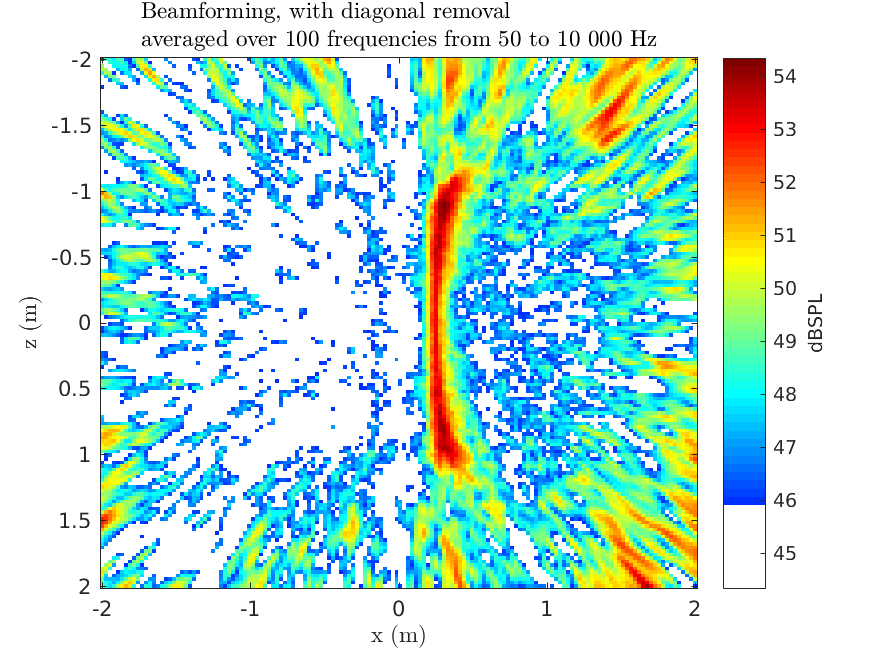
\includegraphics[width = 1\textwidth]{/home/adinsenmey/Bureau/these_2017/Rapports_hebdomadaires/2017_10_11/img/BF_averaged.png}
		\caption{Fonction de Green : monopole}
	\end{subfigure}
	\begin{subfigure}[b]{0.4\textwidth}
		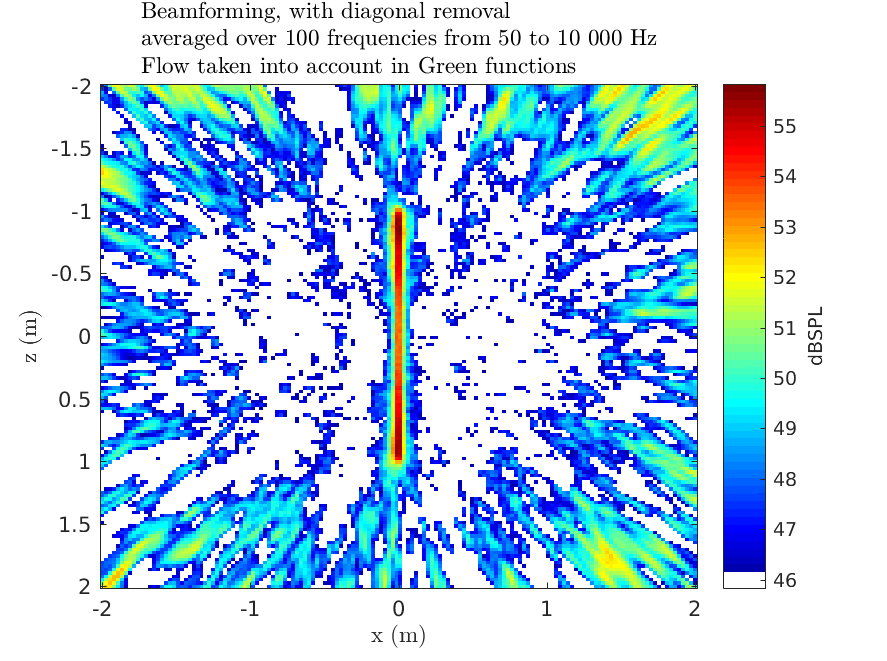
\includegraphics[width = 1\textwidth]{/home/adinsenmey/Bureau/these_2017/Rapports_hebdomadaires/2017_10_11/img/BF_GreenFlow_averaged.png}
		\caption{Fonction de Green : monopole dans un écoulement uniforme}
	\end{subfigure}
	\caption{Comparaison des fonctions de Green sur le cas b1}
	\label{green}
\end{figure*}


\begin{figure*}[h]
	\centering
	\includegraphics[width=0.30\textwidth]{/home/adinsenmey/Bureau/these_2017/Rapports_hebdomadaires/2017_10_11/img/val_propres.png}
	\caption{Valeurs propres de la CSM}
\end{figure*}

\begin{figure*}[h]
	\begin{subfigure}[]{0.3\textwidth}
		\includegraphics[width=\textwidth]{/home/adinsenmey/Bureau/these_2017/Rapports_hebdomadaires/2017_10_11/img/BF_noDG_mean.png}
		\caption{Sur Spp originale}
	\end{subfigure}
	\begin{subfigure}[]{0.3\textwidth}
		\includegraphics[width=\textwidth]{/home/adinsenmey/Bureau/these_2017/Rapports_hebdomadaires/2017_10_11/img/BF_mean_DiagOptim.png}
		\caption{Sur Spp à diagonale optimisée}
	\end{subfigure}
	\begin{subfigure}[]{0.3\textwidth}
		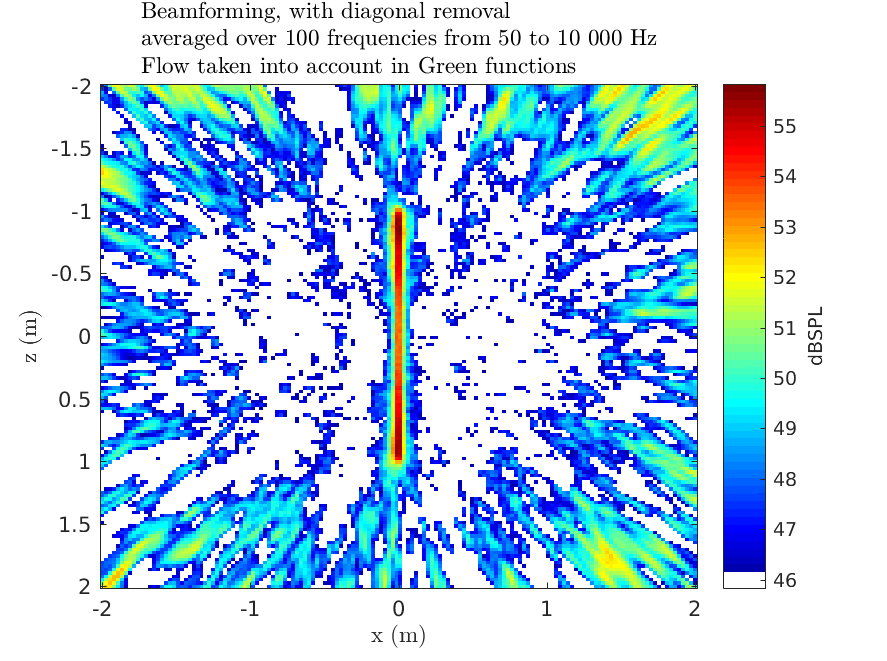
\includegraphics[width=\textwidth]{/home/adinsenmey/Bureau/these_2017/Rapports_hebdomadaires/2017_10_11/img/BF_GreenFlow_averaged.png}
		\caption{Sur Spp à diagonale nulle}
	\end{subfigure}
	\caption{Cartes de beamforming moyennée en fréquences.}
\end{figure*}


\section{Perspectives}
\noindent\begin{minipage}{\columnwidth}
	\begin{itemize}
	\item Correction d'amplitude à appliquer aux points sources en fonction de leur distance par rapport à la position moyenne des microphones
	\item Débruitage de CSM : 
	\begin{itemize}
		\item lire et tester NOVEM Leclère 2015 et Fan Finez 2015
		\item étudier l'impact sur la fft2D de la CSM (lire Petigny 2015)		
\end{itemize}
	\item réfléchir à des critères de validité débruitage/imagerie
	\item Étudier le cas NASA4 (jet) et comparer avec les résultats de C. Bahr
	\item Comparer l'optimisation de diagonale : CVX vs linprog
\end{itemize}
\end{minipage}


\end{document}
